\documentclass[12pt,a4paper,final]{article}
\usepackage{graphicx}
\usepackage[utf8]{inputenc}
\usepackage[german]{babel}
\usepackage{amsmath}
\usepackage{amsfonts}
\usepackage{amssymb}
\author{Eric Gliemmo}
\title{Adaptive Issue Mining Through Data Tracking}
\begin{document}

\title{Adaptive Issue Mining Through Data Tracking\\ - Proposal - }
\author{
\includegraphics[scale=0.3]{Unilogo.png} \\ Eric Gliemmo\\
Universität des Saarlandes \\
Saarbr\"ucken, Deutschland\\
ericgliemmo@online.de
}
\maketitle

\section{Abstract}
These days the analysis of issues of different bug trackers is a remarkable field of application in software mining. Given a dataset of issues of a bug tracking system like BUGZILLA, researchers mine these issues to analyze them and connect them to the source code. One extracts information from the bug reports which are used to predict failures in the concerning program for example. We choose a similar approach, but we want to pursue the mining and don't analyze or evaluate bug tracking systems or its issues itself. To be more accurately, we try to automate the mining process. In fact, we want to create a tool, whereby we are able to generate a miner or a mining plan for an arbitrary bug tracker automatically. \pagebreak 

\section{Problem}
The main problem of mining issues of different bug tracking systems is that they have distinct structure. One tracker uses components which are neglected by another. Or the tracking system uses various scales of classification. For example one bug tracker has five levels to classify the priority of an issue, the other uses only three levels to grade the priority. \\Up to now the common procedure was to mine manually with the help of a spider or a crawler (a computer program that gathers and categorizes information on a website). \\ Hence, there is the next problem of manual issue mining, the changing API (application programming interface) of the issue tracker. Software programs like Redmine or BUGZILLA are always evolving and changing their interface. This fact is very unfavourable for non-adaptive issue miners, because such modifications often remain undetected and the mining software isn't working anymore or the data is not reliable anymore. \\ Furthermore there is no guarantee of the correctness of the mining process. \\ Our proposed solution is an adaptive miner. If we would be able to generate our miner automatically, we would create a robustness and independence against changes of the interface. Effectively themes like 'Tackling Interface Evolution in Issue Tracker for Software Mining' are close to our work. \\ \\ 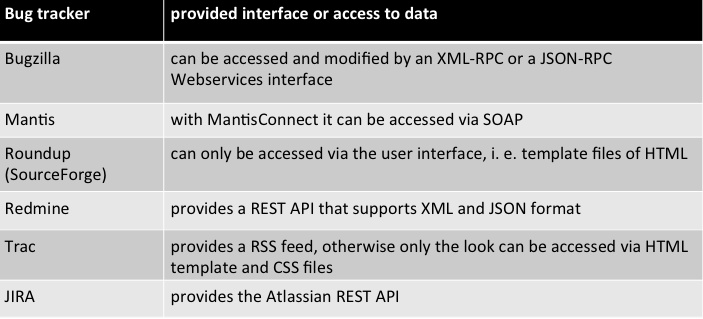
\includegraphics[scale=0.56]{../../../BACHELOR14/Bilder/Folie3.jpg} \\\textbf{Figure 0}: \textit{The most used bug tracking systems and the interface they provide} \\ \\Generally there are various possibilities to access data of bug trackers. The HTML surface, the XML part or the REST (Representational state transfer) API for example are possibilities to extract information. The latter is a method of communication between the user and the server of the bug tracking system. Similar possibilities are XML-RPC (Extensible Markup Language Remote Procedure Call), JSON-RPC (JavaScript Object Notation Remote Procedure Call) and SOAP (Simple Object Access Protocol). RPC means, by sending a HTTP request to a server, that calls a single method of a remote system, one return value is returned. In the case of XML-RPC the input and output format is XML, in the case of JSON-RPC the format is JSON. SOAP is the successor of XML-RPC.  \\ For our case of an adaptive miner, we will decide for the first-mentioned, the HTML surface. All the mentioned capabilities change their  structure in consequence of the changing interface of the bug trackers.  Basically it doesn't matter which opportunity we will choose, because our conceptual approach is adaptive and independent. Nevertheless by using HTML front-end, we can guarantee that all relevant data are available. \\ Figure 1 shows the mentioned changing interface of bug tracking systems as BUGZILLA. In version 4.4 in contrast to version 3.3.4 there are some small, but for bug miners very crucial modifications. For example in 3.3.4 the login fields are visible and the user is able to login directly. In 4.4 the user has to click the login button first, before being able to enter his username and password. These modifications of the HTML structure also influence the information miners want to extract. The location of data could change or, as in our example, an additional link could be necessary for the crawler to access the respective information. \pagebreak
\\ \\ 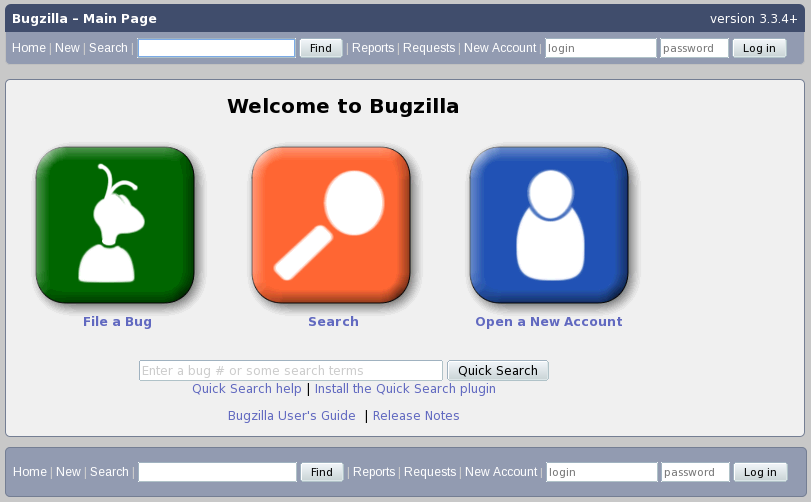
\includegraphics[scale=0.56]{../../../BACHELOR14/Bilder/bugzilla334.png} \\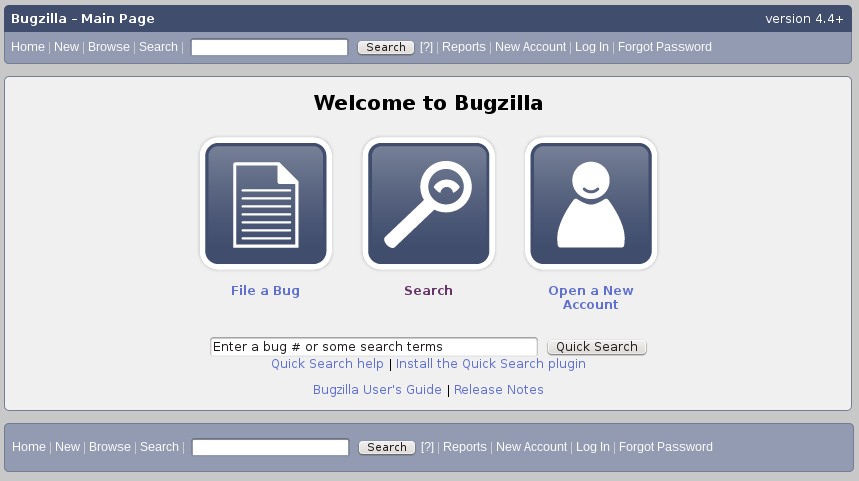
\includegraphics[scale=0.53]{../../../BACHELOR14/Bilder/bugzilla44.png}  \\\textbf{Figure 1}: \textit{As an example of the changing interface of a bug tracking system, the Bugzilla version 3.3.4 on top, at the bottom the version 4.4} \\ \pagebreak

\section{Related Work}
There are similar works concerning mining software repositories. A common method of data mining is the selection of information of bug reports to reference them to the original code. A.Schröder et al. demonstrated two steps in their work 'If Your Bug Database Could Talk...' [1]. First they identified corrections with the message of the fix, which references to the concerning bug report (Fixed \# 3223 for example).\\ Second is, that they mapped bug reports to releases. The version field of the bug database lists the release for which the bug was reported. However they noted that the reliability respectively the trust level is very low. This work leads to the following question: In which parts of the code are the most bugs because of the complexity of the code? Therefore it is necessary to define a metric, that measures the complexity of the code. Such kind of metrics already exist ('Mining metrics to predict
component failures.'[2]), but this research doesn't give a definite answer. The conclusion is, that new metrics or a combination of existing metrics are required to measure the complexity better and more reliably. Consequently this approach of mining bug reports shows the potential of future research based on such bug data.\\ A similar approach chose J.Sliwerski, T.Zimmermann and A.Zeller in their paper 'When Do Changes Induce Fixes?' [3]. They analyzed CVS (Concurrent Versions System) archives for changes that lead to problems, indicated by fixes. They showed how to automatically locate fix-inducing changes by linking a version archive (such as CVS) to a bug database (such as BUGZILLA).\\ 
For the standardization of bug reports there already exists a software called MOZKITO, that realizes these tasks. MOZKITO (developed by Sascha Just and Kim Herzig) models bug reports in a way, that we can abstract all these trackers. So MOZKITO mines reports of different trackers, however not adaptive. Our goal is to develop a tool, that is able to mine bug reports adaptive. Concerning 'related work' there is nothing more to say, because, as seen, there are some earlier approaches in issue mining, but not in the way we are pursuing. 

\section{Contribution}First, we need a standardized view of bug reports. In the paper 'What Makes a Good Bug Report' 2007 [4], Nicolas Bettenburg et al. deal with the question, which information a good bug report would have to contain as well as in their paper 'Quality of Bug Reports in Eclipse' 2007 [5]. \\ Both papers conclude that information on steps to reproduce and stack traces are very important fields of a bug to be a bug report of high quality. The main problem, which resulted in the survey, that was conducted by Bettenburg et al., is the inaccuracy and incompleteness of bug reports. \\ Concerning our approach, this means that we need to define some standards to guarantee that we can compare issues of different bug tracking systems. We have to determine which fields of a bug report are important or significant. In other words, a feature-complete representation of issue reports is desirable. \\ The second point is the reception of a benchmark. To develop our tool, we need to create a set of bug data, which represents the predefined standards in all facets. Partly we will construct this set manually, partly we will extract some existing bug reports from the MOZKITO database. Additionally, this is a basis on which other tools could test their mining results. \\ The third point is our approach of adaptive mining. We will develop a tool, which analyzes the changing structure of reports in different bug tracking systems and generates a corresponding issue miner.  In other words, on the basis of a set of bug reports, our tool yields a mining plan, which states how to extract information of these reports to write them in a database. \\ Given such a tool, we could automatically create issue miner independent from the respective bug tracking systems. In other words, an on-the-fly production of bug tracker miners would be possible, given a way to deploy our created data set. The advantage of our tool, if the deployment would be defective, would be the recognition of this failure during the generating of the miner. The justification therefore is that we have our original data set. If we couldn't mine it with our tool, we would know that something goes wrong. \\ \\ 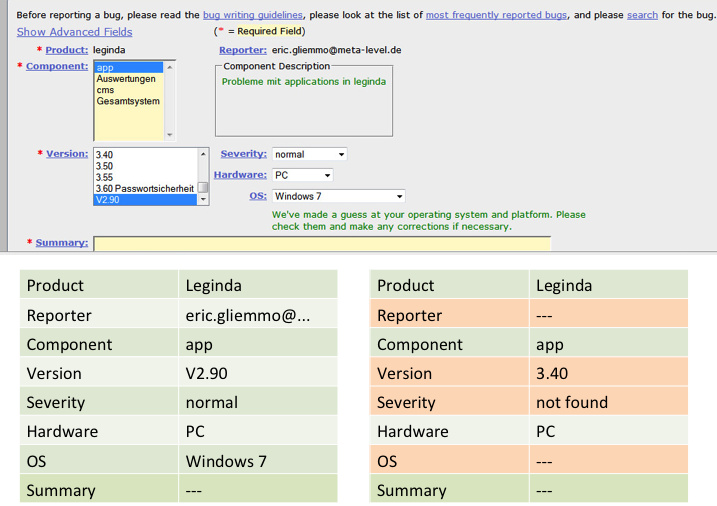
\includegraphics[scale=0.54]{../../../BACHELOR14/Bilder/Folie1.jpg}   \\\textbf{Figure 2}: \textit{On top, a bug report of Bugzilla , on the left the information of our original report and on the right the obtained data after a defective mining process} \\ \\ We can always compare the mining results with our original data and determine if any data was mined wrong or if any data was lost. Furthermore modifications of the interface of bug tracking system would interest no longer. Such failures as shown in Figure 2 could also originate from changing interface of a bug tracker that non-adaptive miners don't recognize.


\section{Methodology}
At first we need a data set in the form of an issue report collection of different bug tracking systems. We will construct a large base of issues that we are able to test our tool on the basis of these data. Our data set has to satisfy several characteristics. For the test purposes at later, it is useful to create those data sets in three different bug tracking systems (BUGZILLA, Jira and SourceForge) and different versions of them to ensure that our tool doesn't work only in a particular case. As mentioned before, this collection will be feature-complete and represent our defined standards. \\ Next we access the HTML surface of our bug reports. HTML (HyperText Markup Language) is the main markup language for creating web pages and other information that can be displayed in a web browser. Tim Berners-Lee, the inventor of the World Wide Web, wrote a memo proposing an Internet-based hypertext system.[6] Berners-Lee specified HTML and wrote the browser and server software in late 1990. The first publicly available description of HTML was a document called "HTML Tags", first mentioned on the Internet by Berners-Lee in late 1991.[7] These days the standard version is HTML 4.01. \\ \\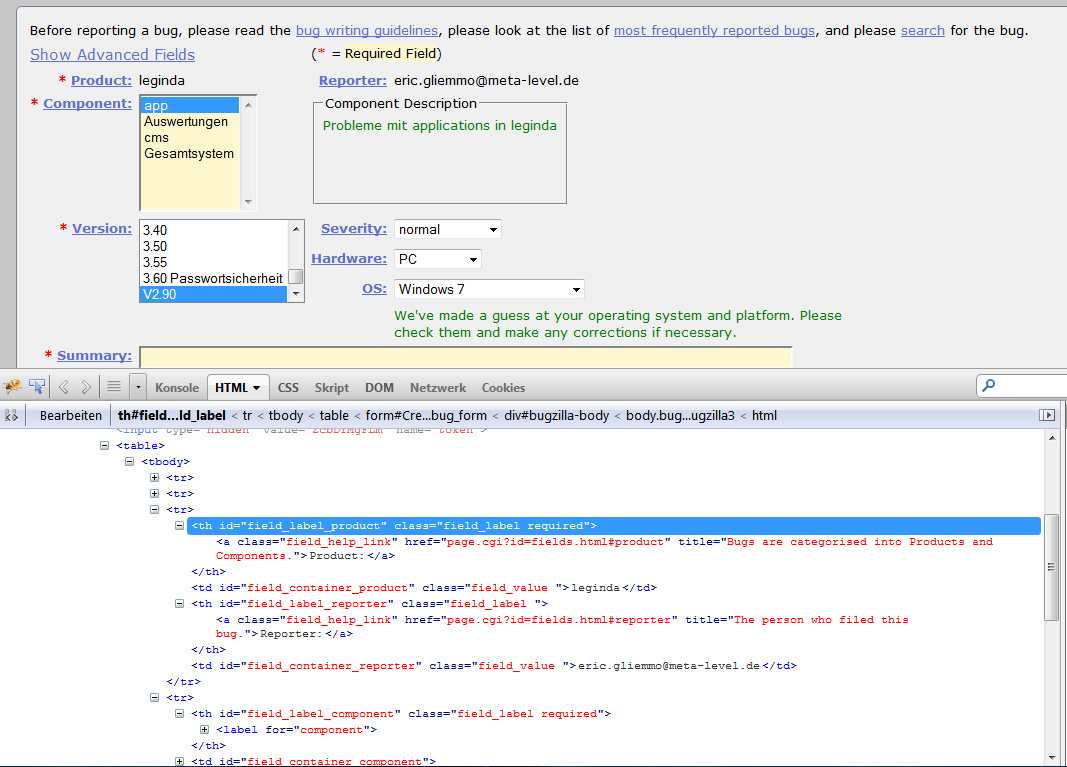
\includegraphics[width=13.8cm,height=13cm]{../../../BACHELOR14/Bilder/Screenshot_bugzilla_html2.jpg}  \\\textbf{Figure 3}: \textit{On the top, a standard Bugzilla bug report in creation, below the HTML code of this report, extracted by Firebug}  \\ \\Tools like Firebug (Figure 3) submit the HTML structure of a website. This structure can be easily converted to XML. Although the HTML and the XML appear very similar, this conversion is necessary. XML (Extensible Markup Language) is also a markup language that defines a set of rules for encoding documents in a format that is human-readable and machine-readable. It is defined in the XML 1.0 Specification produced by the W3C (World Wide Web Consortium), that was also engaged in the development of HTML 4. In contrast to HTML, whose primary purpose is to display data with focus on how the data look, XML is a dynamic language whose primary purpose is the transport and storage of data. That is the reason of our conversion, because we are interested in the containing data of the webpage and not in the design. However, at first glance, the syntax of both languages seems similar. With the use of HTML/XML, we can guarantee the completeness of the data of the website, in contrast to REST, XML-RPC or SOAP, in which this completeness is not secured. A reason therefore is, that HTML is the interface of the biggest target group respectively of the end-user. REST API, XML-RPC or SOAP aren't used by the ordinary user, so they aren't very well maintained and at the most not complete. They are often used only for tools with special assignments. For example the bug tracker MantisBT provides, apart from the HTML surface, SOAP as interface. Therefore the user has to use MantisConnect, a PHP web service that is built on top of Mantis API, that provides an easy way to connect to MantisBT via SOAP.   \\ The next step will be the use of a marker to retrieve our required information. In the XML code of the bug reports we will assign the important fields with markers. In this context the expression 'field' means an information field in a bug report or an issue. For example the priority or the description are such 'fields'. Every field gets a unique sequence of letters, by which we will be able to identify the field and will have a reference to the associated bug report. This marker is important concerning the crawler or spider in later runs. \\After that we put these adapted bug reports in the bug tracking systems mentioned before. Then the crawler or the spider comes to the use. A Web crawler starts with a list of URLs to visit. In our case, this is the URL of the concerning bug report in the bug tracking system. As the crawler visits these URLs, it identifies all the hyperlinks in the page and adds them to the list of URLs to visit next. In a bug report, these are additional information fields or attachments for example that are located on additional sites. Crawlers can validate hyperlinks and HTML code. So if we encounter one of our markers, we have to memorize where we found this marker respectively the associated field. That means that we have to create a mapping that clarifies which field or marker can be found where. So our abortive goal is to obtain a mining plan, that gives an instruction where we can retrieve our desired information. \\ \pagebreak Finally we have got a tool that submits, given some bug reports of a certain bug tracking system, a mining plan to find and select the information of the original bug report and yields these information back for example in the form of database records. 

\section{Evaluation}
After developing our tool, we can test its correctness by applying it to our benchmark set. We will choose a set of random bug reports of our dataset and put them into three different bug tracking systems (BUGZILLA, Jira and SourceForge) and different version of these trackers. Then we will apply our tool to these bug reports and will compare the submitted results with our original data. If we get nearly the same information concerning the data sets after applying our tool, we can say that it is a good adaptive miner. \\ \\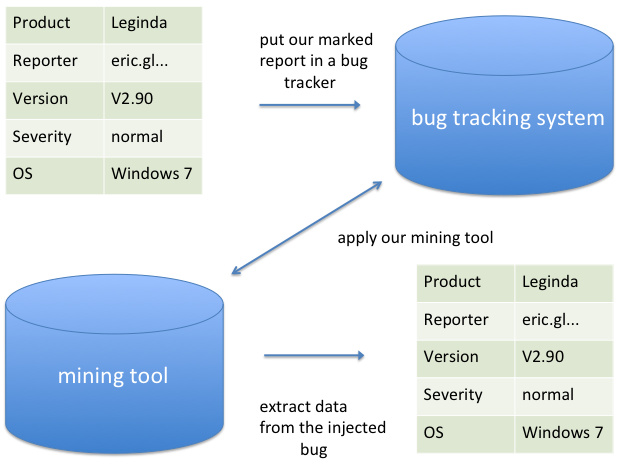
\includegraphics[width=13.8cm,height=10cm]{../../../BACHELOR14/Bilder/Folie2.jpg}  \\\textbf{Figure 4}: \textit{A mining process of our tool without any loss of information.}  \\ \\
Figure 4 shows an optimal mining process. Ensuing from a bug report of our database equipped with our markers, we put this report in a bug tracking system, apply our mining tool and compare the result with our original bug report. We can attest ideal work to our tool if we obtain the same information as result, such as we put it in the bug tracking system. \\ Following problems could appear: On the one hand it is possible that we won't retrieve all information of the original reports. How to handle this problem? Or what could be the reason of this loss of data? Maybe our markers are not precise enough or the crawler does not work as planned. \\ On the other hand, what does it mean, if only two of three bug tracking systems yield good statistics concerning our evaluation of applying the tool?


\section{References}
\begin{enumerate}
\item A.Schröder, T.Zimmermann, Rahul Premraj and A.Zeller. If Your Bug Database Could Talk... In Proceedings of the 5th International Symposium on Empirical Software Engineering, ISESE 2006. 
\item N. Nagappan, T. Ball, and A. Zeller. Mining metrics to predict
component failures. In Proceedings of the International
Conference on Software Engineering, ICSE 2006.
\item J. Sliwerski, T. Zimmermann and A. Zeller. When do changes
induce fixes? In Proc. International Workshop on Mining
Software Repositories (MSR), St. Louis, Missouri, U.S., May
2005.
\item N. Bettenburg, S. Just et al. What Makes a Good Bug Report? Universität des Saarlandes, Saarbrücken, Germany, March 2008. 
\item N. Bettenburg, S. Just et al. Quality of Bug Reports in Eclipse. Proceedings of the 2007 OOPSLA Workshop on Eclipse Technology eXchange, ACM Press, New York, NY, USA, October 2007. 
\item Tim Berners-Lee. Information Management: A Proposal. CERN (March 1989, May 1990).
\item Tim Berners-Lee. First mention of HTML Tags on the www-talk mailing list. World Wide Web Consortium. October 29, 1991.
\end{enumerate}
\end{document}